\documentclass[12pt, twoside]{article}
\usepackage[utf8]{inputenc}
\usepackage[english,russian]{babel}
\newcommand{\hdir}{.}

\usepackage{graphicx}
\usepackage{caption}
\usepackage{amssymb}
\usepackage{amsmath}
\usepackage{mathrsfs}
\usepackage{euscript}
\usepackage{upgreek}
\usepackage{array}
\usepackage{theorem}
\usepackage{graphicx}
\usepackage{subfig}
\usepackage{caption}
\usepackage{color}
\usepackage{url}

\usepackage[left=2cm,right=2cm,top=3cm,bottom=2cm,bindingoffset=0cm]{geometry}

\usepackage{fancyhdr}
\pagestyle{fancy}
\fancyhead{}
\fancyhead[LE,RO]{\thepage} 
\fancyhead[CO,CE]{Лекция 4}
\fancyhead[LO,LE]{Грабовой Андрей}

\begin{document} 

\begin{center}
{\LARGE\bf
Основные структуры данных
}
\end{center}

\section{Список}
\begin{itemize}
	\item Каждый элемент знает только свое значение.
	\item Каждый элемент знает где находиться следующий элемент списка.
	\item* В случае двусвязного списка каждый элемент знает где находится предыдущий элемент.
\end{itemize}

\begin{figure}[h!t]\center
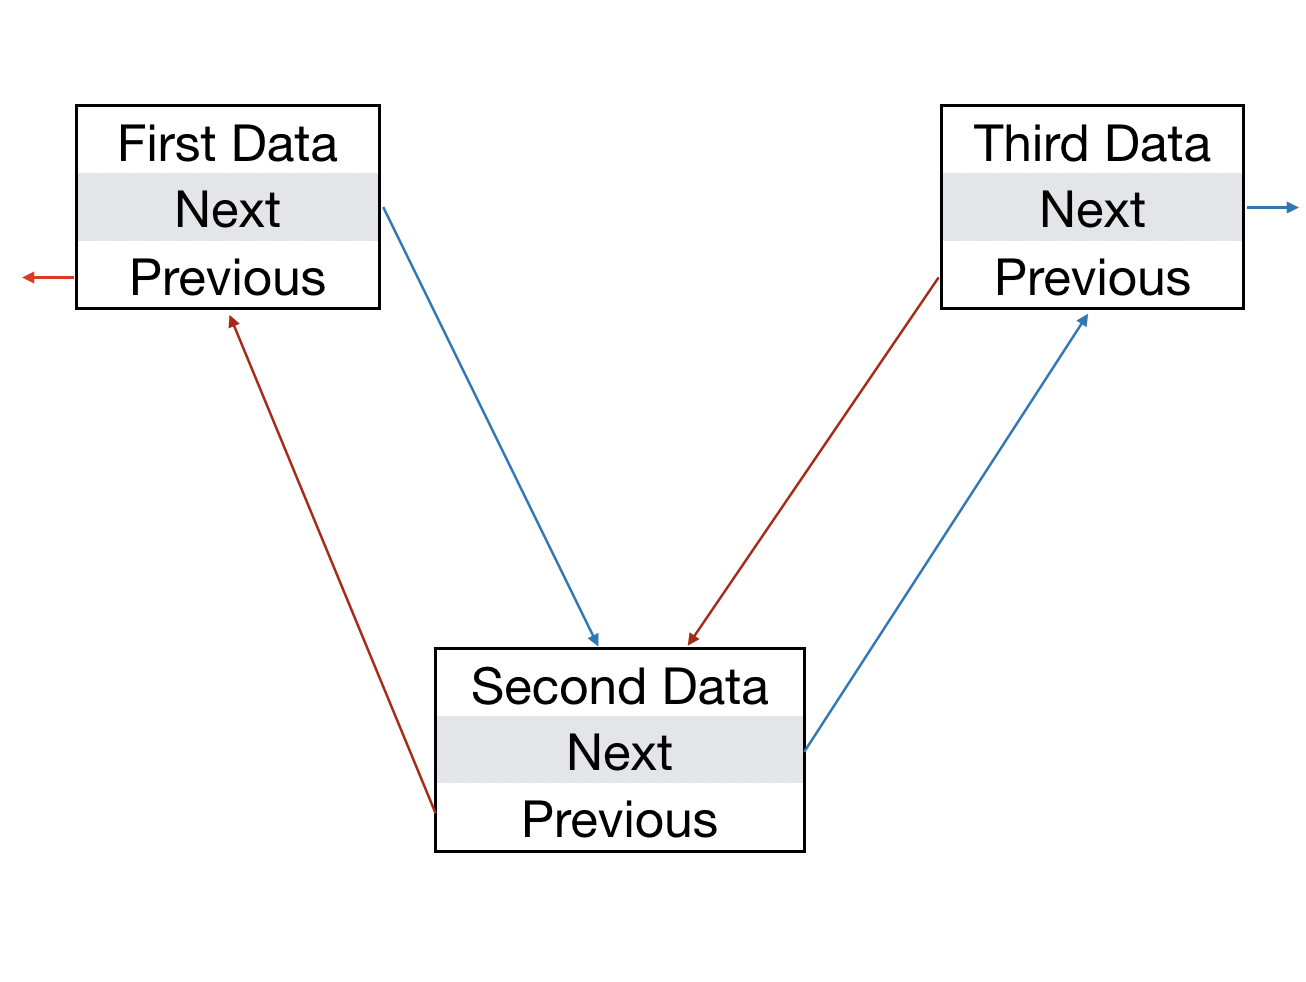
\includegraphics[width=0.6\textwidth]{Lecture_4_List.jpg}
\caption{Изображение списка}
\label{Lecture_4_List}
\end{figure}

На рис.~\ref{Lecture_4_List} изображена общая структура списка. Если на рис.~\ref{Lecture_4_List} оставить только синие линии то получим простой список, если же оставить все линии, то получаем двусвязный список.\\

Основные операции:
\begin{itemize}
	\item append() --- добавить в конец списка,
	\item pop(index)  --- вытащить элемент со списка с индексом index,
	\item len() --- возвращает длину списка.
\end{itemize}

\section{Стэк}
\begin{itemize}
	\item Главное свойство, кто первый попадает в стэк, тот последним из него выходит.
\end{itemize}

\begin{figure}[h!t]\center
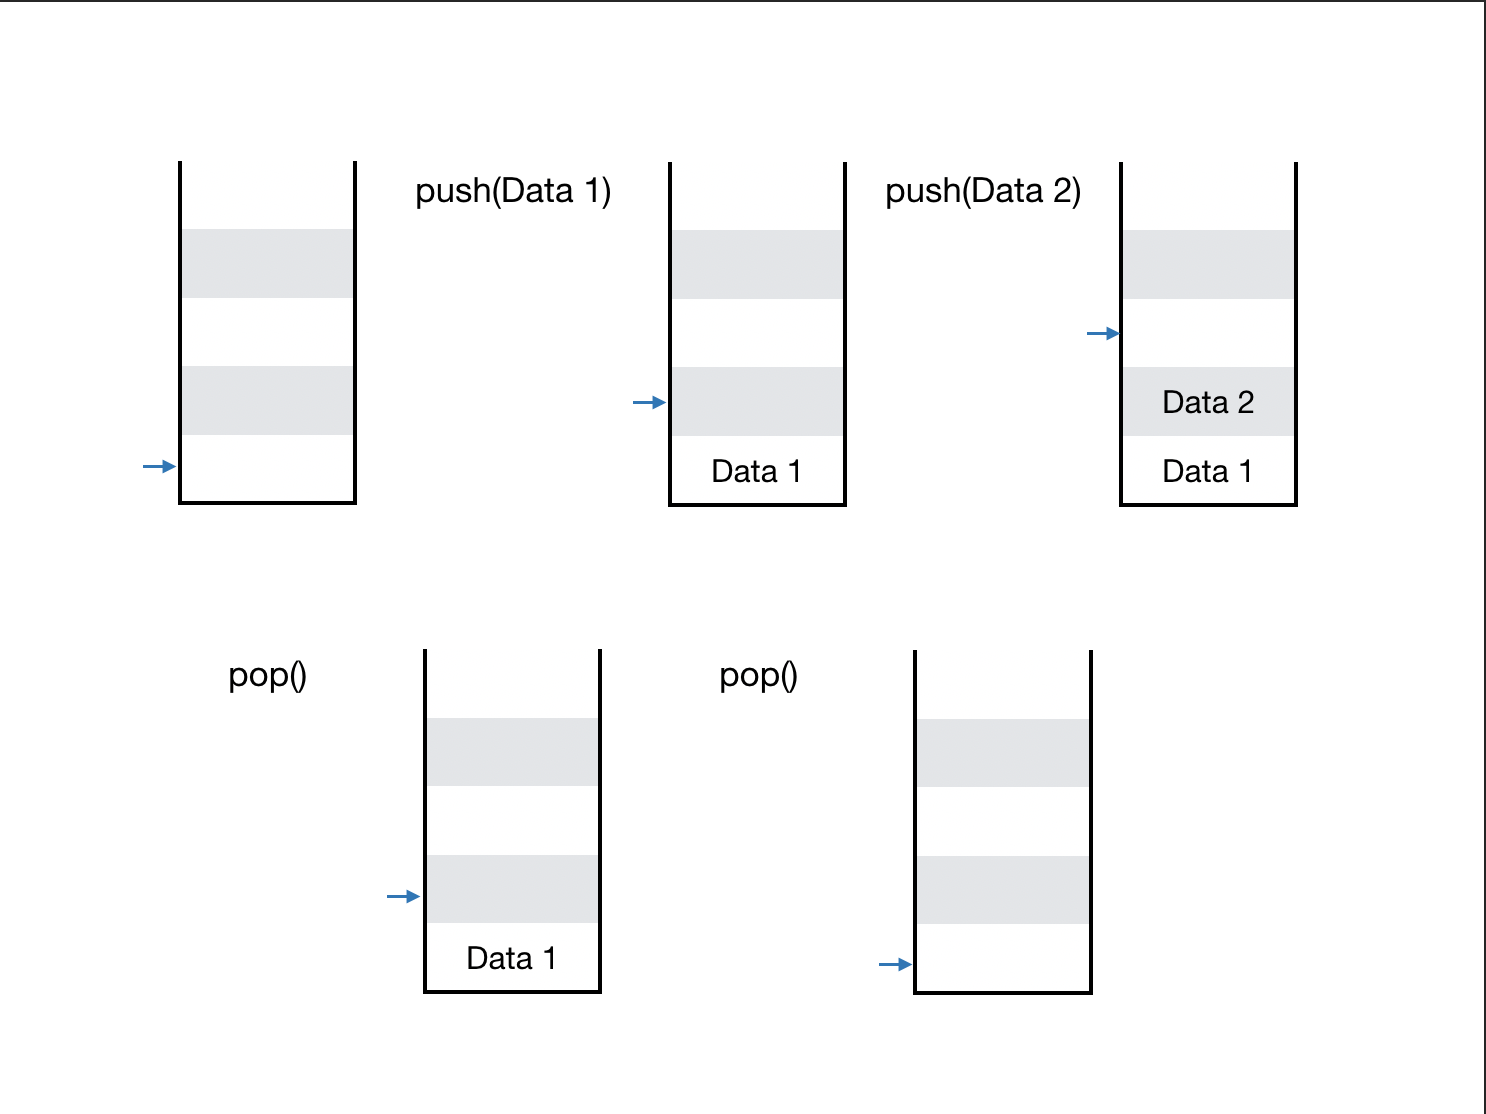
\includegraphics[width=0.6\textwidth]{Lecture_4_Stek.jpg}
\caption{Изображение стэка}
\label{Lecture_4_Stek}
\end{figure}

На рис.~\ref{Lecture_4_Stek} изображена общая структура стэка. Как видно сначала из стэка достается элемент который в него был поставлен в самом конце и последним достается элемент который был поставлен первым. На рис.~\ref{Lecture_4_Stek}  синяя стрелочка указывает, на место куда будет вставлен следующий элемент и какой элемент будет изъят следующим.\\

Основные операции:
\begin{itemize}
	\item push() --- добавить в вверх стэка,
	\item pop()  --- вытащить верхний элемент стэка,
	\item len() --- возвращает глубину стэка.
\end{itemize}

\section{Очередь}
\begin{itemize}
	\item Главное свойство, кто первый попадает в очередь, тот первым из нее выходит в отличии от стэка.
\end{itemize}


\begin{figure}[h!t]\center
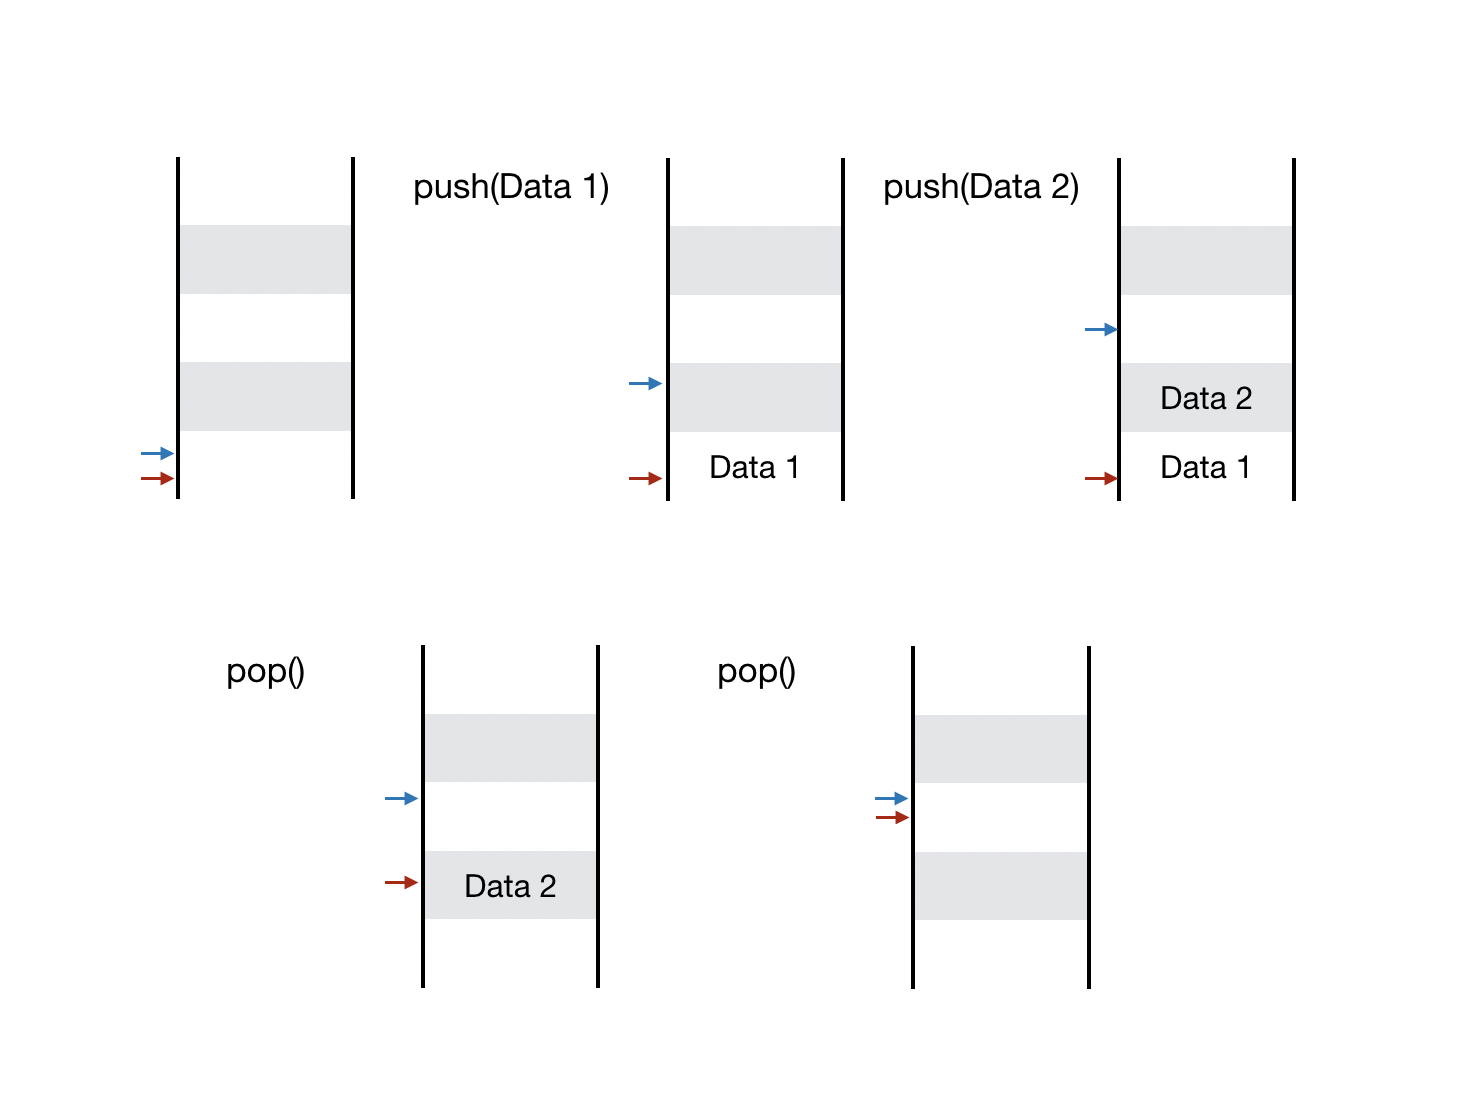
\includegraphics[width=0.6\textwidth]{Lecture_4_Queue.jpg}
\caption{Изображение стэка}
\label{Lecture_4_Queue}
\end{figure}

На рис.~\ref{Lecture_4_Queue} изображена общая структура очереди. Синяя срелочка показывает в какое место будет вставлен следующий элемент, а красная стрелочка указывает откуда будет браться следующий элемент. Как видно, первый элемент который попал в очередь первый из нее выходит.\\

Основные операции:
\begin{itemize}
	\item push() --- добавить в конец очередь,
	\item pop()  --- вытащить первый элемент очереди,
	\item len() --- возвращает длину очереди
\end{itemize}


\section{Set}
\begin{itemize}
	\item Это структура данных, которая отвечает такой математической структуре как множество.
	\item Главная задача этой структуры, это ответить на вопрос есть ли элемент в множестве.
	\item В отличии от структур 1---3 эта структура не имеет порядка.
\end{itemize}

Основные операции:
\begin{itemize}
	\item insert() --- добавить элемент в множество,
	\item find()  --- найти элемент в множестве,
\end{itemize}

Операция find() вернет либо $0$ либо $1$ в зависимости от того, принадлежит элемент множеству или нет.

\section{Map}
\begin{itemize}
	\item map и set очень похожие структуры данных.
	\item map отличается от set, только тем, что в нем храниться не только информация есть ли элемент а еще и каждому элементу ставиться в соответствии еще один элемент.
	\item Каждая пара состоит из key и data, где key должен быть уникальным.
\end{itemize}

Пример использования map очень просто, например мы хотим сделать перепись книг в библиотеке. В качестве уникальных key будет выступать название книги, а в качестве data будет выступать числа книг соответствующих этому названию.

\section{Hash}
\begin{itemize}
	\item Хэш таблица --- способ хранения данных
	\item Нужна hash функция для данных которые вы собираетесь хранить
\end{itemize}

Хэш таблица это просто массив фиксированного размера в котором хранятся некоторые данные, но доступ к этим данным происходит не по простой индексации, а при помощи hash функции.\\

Hash функция это некоторое отображения данных которые нужно сохранить в натуральное число --- индекс массива.

Основной минус, что количество данных обычно много больше чем размер массива, поэтому на самом деле элемент массива это список тех элементов у которых Hash функция дает один и тот же результат. Список решает проблему так называемой коллизии.








\end{document} 